\documentclass[11pt]{article}
\usepackage[margin=1in]{geometry}
\usepackage{amsmath,amssymb,amsthm}
\usepackage{graphicx}
\usepackage{enumitem}
\usepackage{booktabs}
\usepackage[hidelinks]{hyperref}
\usepackage{caption}
\captionsetup{font=small,labelfont=bf}

\newtheorem{theorem}{Theorem}
\newtheorem{lemma}{Lemma}
\newtheorem{proposition}{Proposition}
\newtheorem{corollary}{Corollary}
\theoremstyle{definition}
\newtheorem{definition}{Definition}
\newtheorem{remark}{Remark}

\newcommand{\Z}{\mathcal{Z}}
\newcommand{\F}{\mathcal{F}}
\newcommand{\X}[1]{X_{#1}}

\title{\vspace{-1.2em}Locality of $\mathrm{Tr}(\phi^3)$ tree amplitudes from cyclic hidden zeros\\[2pt]
\large Part II: the fat--zero generalisation}
\date{}
\author{}

\begin{document}
\maketitle
\vspace{-3.2em}

\begin{abstract}
\noindent Part I established locality through $n=9$ by combining a single asymptotic ``kill'' on
one hidden $1$--zero with a per--$n$ Laurent cascade. Here we promote the $1$--zero to a
\emph{$k$--zero} (``fat zero''): the simultaneous imposition of the hidden--zero relations on $k$
consecutive boundaries. A $k$--zero kills strictly more nonlocal coefficients than the $1$--zero. We
derive its constraint surface and classify, by a rate--vector analysis, all admissible asymptotic
limits in which the special chord diverges---i.e.\ the criteria $A$, $B$, $C$ promised in the title.
The geometric shadow of these limits is the construction of a $(k{+}2)$--gon on top of the
length--$k$ enclosing chord; we show there are three flavours of completion (special, bare, and an
internal \emph{column pair}). These criteria are the correct objects; the open problem is to
assemble them, across all zeros, into an all--$n$ proof. The Step--$2$ coefficient equations, now
classified for the $1$--, $2$--, and $3$--zeros, are the tool for that assembly and are documented
in Part III.
\end{abstract}

\section{From one zero to many}
We keep the conventions of Part I. The $n$--gon has vertices $1,\dots,n$; a chord $\X{ij}$
($1\le i<j\le n$, $|j-i|\ne 1$, $(i,j)\ne(1,n)$) is a variable; an edge $\X{m,m+1}$ is a leg and
equals $0$. The ansatz is $B_n=\sum_{|M|=n-3} a_M\big/\prod_{c\in M}\X{c}$ over multisets $M$, and
locality is the statement $a_M=0$ whenever $M$ contains a crossing pair.

A cyclic hidden \emph{$1$--zero} imposes the $n-3$ relations $c_{1j}=0$, where
\begin{equation}\label{eq:c}
  c_{ij} \;=\; \X{ij}+\X{i+1,\,j+1}-\X{i,\,j+1}-\X{i+1,\,j}.
\end{equation}
On $\Z_{1,3}$ these read $\X{2k}=\X{1k}-\X{13}$ and $\X{2n}=-\X{13}$; the special chord is $\X{13}$
and the bare chord is $\X{2n}$.

\begin{definition}[$k$--zero]\label{def:kzero}
For $1\le k\le n-3$, the \emph{$k$--zero based at $\{1,\dots,k{+}1\}$} is the simultaneous imposition
\begin{equation}\label{eq:kzero}
  c_{ij}=0,\qquad i=1,\dots,k,\quad j=k+2,\dots,n-1 .
\end{equation}
\end{definition}
\noindent It collects the hidden--zero relations on the $k$ consecutive boundaries
$(1,2),(2,3),\dots,(k,k{+}1)$. For $k=1$ it is the ordinary $1$--zero. There are $k(n-k-2)$
relations, and they cut out a linear surface $\Z^{(k)}$ that we now describe explicitly.

\section{The constraint surface of a $k$--zero}
\begin{lemma}[Telescoping]\label{lem:tele}
On $\Z^{(k)}$, with the leg convention $\X{m,m+1}=0$,
\begin{align}
  \X{k+1,\,j} &= \X{1j}-\X{1,k+2}, & j&=k+3,\dots,n-1; & \X{k+1,\,n}&=-\X{1,k+2}, \label{eq:backbone}\\
  \X{ij} &= \X{k+1,\,j}+\X{i,\,k+2}, & i&=2,\dots,k,\ \ j=k+3,\dots,n. \label{eq:interior}
\end{align}
\end{lemma}
\begin{proof}
Sum \eqref{eq:c} over the full block of rows $i=1,\dots,k$ at fixed $j$. The two inner sums
telescope and leave $\sum_{i=1}^{k}c_{ij}=\big(\X{1j}-\X{k+1,j}\big)-\big(\X{1,j+1}-\X{k+1,j+1}\big)=0$,
so $\X{k+1,j}-\X{1j}$ is independent of $j$. Evaluating at $j=k+2$ (where $\X{k+1,k+2}=0$) gives the
constant $-\X{1,k+2}$, which is \eqref{eq:backbone}; at $j=n$ one has $\X{1n}=0$, giving the bare
relation. Summing instead the partial block $i'=i,\dots,k$ gives
$\X{ij}-\X{i,j+1}=\X{k+1,j}-\X{k+1,j+1}$; telescoping this in $j$ from $k+2$ (where
$\X{k+1,k+2}=0$) yields \eqref{eq:interior}.
\end{proof}

\noindent Three structures organise $\Z^{(k)}$ (Figure~\ref{fig:geometry}).
\begin{itemize}[topsep=2pt,itemsep=1pt]
  \item The \textbf{near block} $N=\{1,\dots,k{+}1\}$ and the \textbf{far block}
  $F=\{k{+}2,\dots,n\}$. Every chord internal to $N$ or to $F$ is absent from \eqref{eq:kzero}: these
  are the \emph{born--free} chords, untouched by the $k$--zero.
  \item The length--$k$ \textbf{enclosing chord} $\X{1,k+1}$ closes the $k$ consecutive boundaries
  into the $(k{+}1)$--gon $N$. It is born--free.
  \item The \textbf{special} $\X{1,k+2}$ and the \textbf{bare} $\X{k+1,n}$, the exact analogues of
  $\X{13}$ and $\X{2n}$: each bridges $N$ to $F$ across one boundary of $N$.
\end{itemize}
All remaining constrained chords are \emph{bridges} from a near vertex to a far vertex, grouped into
\emph{columns} indexed by the far endpoint $j$: column $j$ is $\{\X{1j},\X{2j},\dots,\X{k+1,j}\}$.
By Lemma~\ref{lem:tele} a column is fixed by the single free choice $\X{1j}$ together with the shared
offsets $\X{1,k+2}$ (special) and $\X{i,k+2}$ ($i=2,\dots,k$). A convenient independent coordinate
system on $\Z^{(k)}$ is therefore
\begin{equation}\label{eq:coords}
  \underbrace{\{\X{1,k+2}\}}_{\text{special }s}\ \cup\
  \underbrace{\{\X{i,k+2}:2\le i\le k\}}_{\text{column-}(k+2)\text{ offsets}}\ \cup\
  \underbrace{\{\X{1\ell}: k+3\le \ell\le n-1\}}_{\text{one per far column}}\ \cup\ \{\text{born--free}\},
\end{equation}
of which the $n-3$ bridge coordinates determine every constrained chord.

\begin{figure}[t]
  \centering
  
\includegraphics[width=0.38\textwidth]{figures/geometry.pdf}
  \caption{Geometry of a $k$--zero ($n=10$, $k=3$). Near block $N=\{1,2,3,4\}$ (gold), far block
  $F=\{5,\dots,10\}$ (blue). Green: the length--$k$ enclosing chord $\X{1,4}$. Red dashed: the special
  $\X{1,5}$. Blue dashed: the bare $\X{4,10}$. Born--free chords live inside $N$ or inside $F$.}
  \label{fig:geometry}
\end{figure}

\section{The kill: a rate--vector classification}\label{sec:kill}
The kill mechanism is the Laurent argument of Part~I. A one--parameter limit on $\Z^{(k)}$ sends
some chords to infinity; the terms whose denominators remain finite form a vanishing Laurent
polynomial in the finite coordinates, so $a_M=0$ for every $M$ supported on the finite set $\F$.

What is special about the $k$--zero is that the surface $\Z^{(k)}$ admits a rich family of such
limits, and the constraints \eqref{eq:backbone}--\eqref{eq:interior} couple the chords, so we are
\emph{not} free to hold an arbitrary subset finite. We parametrise the limits exactly. Fix a divergent
parameter $s\to\infty$ (the special) and assign each remaining bridge coordinate a leading rate:
\begin{equation}\label{eq:ratevec}
  \X{i,k+2}\;\sim\;\beta_i\,s\ (i=2,\dots,k),\qquad
  \X{1\ell}=u_\ell\;\sim\;\alpha_\ell\,s\ (\ell=k+3,\dots,n-1),
\end{equation}
with $\alpha_\ell,\beta_i\in\mathbb{R}$ and equality of leading coefficients understood. Each chord
on $\Z^{(k)}$ then has a definite rate, read off from \eqref{eq:backbone}--\eqref{eq:interior}:
\begin{equation}\label{eq:chordrates}
\renewcommand{\arraystretch}{1.15}
\begin{array}{l|l|l}
\textnormal{chord} & \textnormal{rate} & \textnormal{finite iff} \\ \hline
\X{1\ell}                          & \alpha_\ell\,s              & \alpha_\ell=0 \\
\X{k+1,\ell}\!=\!u_\ell-s          & (\alpha_\ell-1)\,s          & \alpha_\ell=1 \\
\X{i\ell}\!=\!u_\ell-s+\X{i,k+2}   & (\alpha_\ell+\beta_i-1)\,s  & \alpha_\ell+\beta_i=1 \\
\X{i,k+2}                          & \beta_i\,s                  & \beta_i=0 \\
\X{in}\!=\!\X{i,k+2}-s             & (\beta_i-1)\,s              & \beta_i=1 \\
\X{1,k+2}\!=\!s                    & s                           & \textnormal{\emph{never}} \\
\X{k+1,n}\!=\!-s                   & -s                          & \textnormal{\emph{never}}
\end{array}
\end{equation}
Each rate vector $(\alpha_\ell;\beta_i)$ thus determines an admissible finite--set
\begin{equation}\label{eq:Fdef}
  \F(\alpha,\beta)\;=\;\{\text{born--free}\}\ \cup\ \{\text{the chords whose ``finite iff'' clause in
  \eqref{eq:chordrates} holds}\}.
\end{equation}

\begin{theorem}[Admissible finite--sets]\label{thm:rates}
Every admissible finite--set on $\Z^{(k)}$ based at $\{1,\dots,k{+}1\}$ has the form
$\F(\alpha,\beta)$ for some $(\alpha_\ell;\beta_i)\in\mathbb{R}^{(n-k-3)+(k-1)}$. The special
$\X{1,k+2}$ and the bare $\X{k+1,n}$ are absent from every $\F(\alpha,\beta)$. Consequently
\begin{equation*}
  a_M\;=\;0\qquad\text{whenever }\ M\subseteq\F(\alpha,\beta)\ \text{for some }(\alpha,\beta).
\end{equation*}
\end{theorem}
\begin{proof}
Every limit on $\Z^{(k)}$ is determined by the leading scaling of the independent coordinates
\eqref{eq:coords}; \eqref{eq:ratevec} captures this for the bridges, the born--free coordinates are
held finite. The rate of each remaining chord is given by
\eqref{eq:backbone}--\eqref{eq:interior}, and is finite precisely under the listed condition. The
Laurent--polynomial vanishing on the finite coordinates then forces $a_M=0$ for $M\subseteq\F$. The
special and bare carry an uncancellable bare power of $s$.
\end{proof}

The named regimes are the three structurally distinct ways of fixing the rate vector:

\smallskip
\begin{tabular}{@{}p{0.16\textwidth}p{0.40\textwidth}p{0.40\textwidth}@{}}
\toprule
\textbf{(A) 1--side} & all $\beta_i=0$ and all $\alpha_\ell=0$. & $\F_A=\{\X{i,k+2}:2\le i\le k\}\cup\{\X{1\ell}:k{+}3\le\ell\le n{-}1\}$. \\[2pt]
\textbf{(B) $(k{+}1)$--side} & all $\beta_i=1$ and all $\alpha_\ell=1$. & $\F_B=\{\X{in}:2\le i\le k\}\cup\{\X{k+1,\ell}:k{+}3\le\ell\le n{-}1\}$. \\[2pt]
\textbf{(C) mixed} & any other consistent rate vector. & per--column slot picks plus offset pairings, as dictated by \eqref{eq:chordrates}. \\
\bottomrule
\end{tabular}
\smallskip

\begin{figure}[t]
  \centering
  \begin{minipage}[t]{0.40\textwidth}\centering
    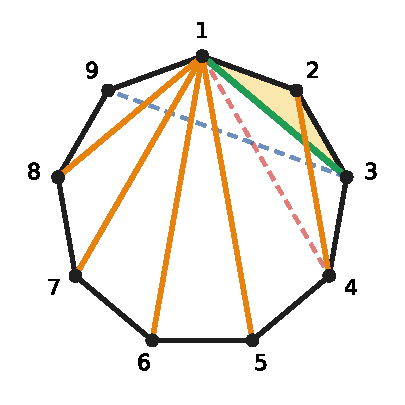
\includegraphics[width=\textwidth]{figures/regimeA.pdf}\\[-1pt]
    {\footnotesize Regime $A$}
  \end{minipage}\hfill
  \begin{minipage}[t]{0.40\textwidth}\centering
    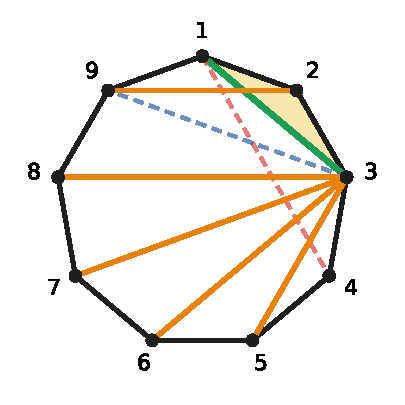
\includegraphics[width=\textwidth]{figures/regimeB.pdf}\\[-1pt]
    {\footnotesize Regime $B$}
  \end{minipage}
  \caption{The held--finite bridges (orange) for the two homogeneous regimes, $n=9$, $k=2$
  (special/bare faint dashed, enclosing chord green). $A$ keeps the $1$--side
  $\{\X{24};\X{15},\X{16},\X{17},\X{18}\}$; $B$ keeps the $(k{+}1)$--side
  $\{\X{29};\X{35},\X{36},\X{37},\X{38}\}$. Both are special cases of Theorem~\ref{thm:rates}.}
  \label{fig:AB}
\end{figure}

\noindent
$A$ and $B$ are homogeneous: setting all the $\alpha$'s and $\beta$'s to the same value finitises
exactly one slot per column. $C$ is everything else---e.g.\ taking $\beta_i=0$ but $\alpha_\ell=1$
for some $\ell$ makes \emph{both} $\X{k+1,\ell}$ and $\X{i\ell}$ finite, a paired configuration not
seen in either homogeneous regime. Figure~\ref{fig:C} shows the canonical per--column three slots
that organise the $C$ family (one finite chord per column, before pairings); the full $C$ family is
the family of all rate vectors compatible with the chosen $\F$ via \eqref{eq:chordrates}.

\begin{figure}[t]
  \centering
  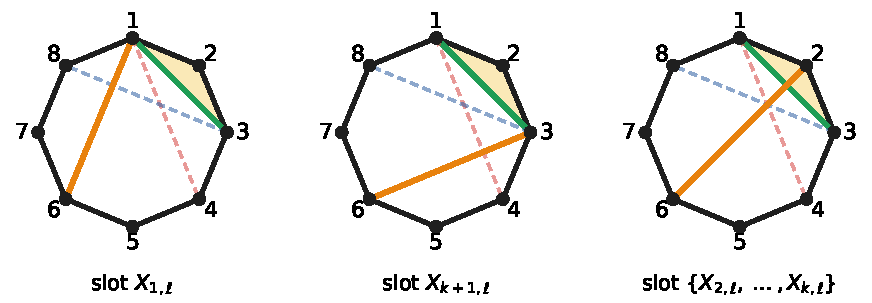
\includegraphics[width=0.95\textwidth]{figures/criterionC.pdf}
  \caption{Regime $C$: the three exclusive \emph{single--chord} slots per far column, here $\ell=6$,
  $n=8$, $k=2$. Each rate vector $(\alpha,\beta)$ picks one per column, and---via the offset rates
  $\beta_i$---may simultaneously pair additional interior bridges $\X{i\ell}$ into $\F$.}
  \label{fig:C}
\end{figure}

\section{The geometry: $(k{+}2)$--gons over the enclosing chord}\label{sec:geom}
Theorem~\ref{thm:rates} has a clean geometric shadow when restricted to multisets that do not cross
the enclosing chord.

\begin{proposition}[$(k{+}2)$--gon survival]\label{prop:kgon}
Let $M$ be a multiset using no chord that crosses $\X{1,k+1}$. Then $M$ survives the $k$--zero based
at $\{1,\dots,k{+}1\}$ if and only if $M$ contains a $(k{+}2)$--gon completion of the near block $N$:
exactly one of
\begin{enumerate}[label=\textnormal{(\roman*)},topsep=2pt,itemsep=1pt]
  \item the special $\X{1,k+2}$ (closing $N$ into $\{1,\dots,k{+}2\}$);
  \item the bare $\X{k+1,n}$ (closing $N$ into $\{n,1,\dots,k{+}1\}$);
  \item a \emph{column pair} $\{\X{1m},\X{k+1,m}\}$ for some $m\in\{k{+}3,\dots,n{-}1\}$ (closing
        $N$ into $\{1,\dots,k{+}1,m\}$).
\end{enumerate}
See Figure~\ref{fig:kgon}. Each completion is the unique way to extend $N$ to a $(k{+}2)$--gon
across exactly one further polygon boundary.
\end{proposition}
\begin{proof}
Under the no--crossing hypothesis every bridge in $M$ has near endpoint $1$ or $k{+}1$, i.e.\ is of
the form $\X{1j}$, $\X{k+1,j}$ (including the special $\X{1,k+2}$ and the bare $\X{k+1,n}$).
$M$ survives iff no rate vector $(\alpha,\beta)$ finitises every chord of $M$. By
\eqref{eq:chordrates} the conditions imposed by $M$'s bridges are: $\alpha_\ell=0$ for each
$\X{1\ell}\in M$ with $\ell\in\{k{+}3,\dots,n{-}1\}$, $\alpha_\ell=1$ for each $\X{k+1,\ell}\in M$,
and (impossible) clauses for special and bare. The constraint system is inconsistent precisely when
one of (i)--(iii) holds: the special or the bare forces an impossible $1{=}0$ clause; a column pair
forces $\alpha_m{=}0$ and $\alpha_m{=}1$. Conversely if none of (i)--(iii) holds, the system is
consistent (set $\alpha_\ell=0$ where $\X{1\ell}\in M$, $\alpha_\ell=1$ where $\X{k+1,\ell}\in M$,
any value elsewhere; $\beta_i$ free), so $M\subseteq\F(\alpha,\beta)$ and is killed. The
$(k{+}2)$--gons containing $N$ are exactly $\{1,\dots,k{+}1,m\}$ for $m\in F$, and each is closed by
the chord(s) in (i)--(iii).
\end{proof}

\begin{figure}[t]
  \centering
  
\includegraphics[width=0.95\textwidth]{figures/kplus2gon.pdf}
  \caption{The three $(k{+}2)$--gon completions of $N$ ($n=10$, $k=3$, $m=8$ for the column pair).
  In every non--crossing survivor, exactly one of these occurs.}
  \label{fig:kgon}
\end{figure}

The complete (crossing--allowed) survival criterion is the linear--algebra contrapositive of
\eqref{eq:chordrates}: $M$ survives iff the system of rate equations imposed by the chords of $M$ is
inconsistent in $(\alpha_\ell,\beta_i)$. Geometrically the simplest non--$(k{+}2)$--gon survival
modes are pairings of bridges that share a far vertex from the offsets (e.g.\ $\{\X{i,k+2},\X{in}\}$
forcing $\beta_i=0$ and $\beta_i=1$), or longer cycles of incompatible rate constraints.

\section{Survivors}\label{sec:survivors}
\begin{figure}[h]
  \centering
  
\includegraphics[width=0.97\textwidth]{figures/survivors.pdf}
  \caption{Three families of survivors of the $k=2$ zero based at $\{1,2,3\}$, $n=8$. (a) The
  special $\X{1,4}$ is present (the simplest $(k{+}2)$--gon completion). (b) A column pair
  $\{\X{1,6},\X{3,6}\}$ forces $\alpha_6{=}0$ and $\alpha_6{=}1$ simultaneously. (c) An offset pair
  $\{\X{2,4},\X{2,8}\}$ forces $\beta_2{=}0$ and $\beta_2{=}1$ simultaneously. In every case the
  rate--equation system is inconsistent, so no admissible $\F$ contains $M$.}
  \label{fig:survivors}
\end{figure}

\noindent A triangulation always escapes the $k$--zero: if the $(k{+}1)$--gon over $k$ consecutive
edges is self--contained (no chord of the triangulation crosses the enclosing chord
$\X{1,k+1}$), then adjoining $\X{1,k+1}$ crosses nothing, so it is already a chord of the
triangulation, and---being a chord of a triangulation---bounds a triangle on its far side, supplying
a $(k{+}2)$--gon completion. By Proposition~\ref{prop:kgon} the triangulation survives.

The conjecture of the program is that, ranging over all $k$ and all cyclic rotations, the union of
the $k$--zero kills removes every non--triangulation, so that exactly the triangulations survive.

\section{Status and the road ahead}\label{sec:status}
Theorem~\ref{thm:rates} is the corrected statement of the kill: the survival criteria
$A$, $B$, $C$ are the three structural cases of a single rate--vector classification, derived
rigorously from the coupling \eqref{eq:backbone}--\eqref{eq:interior}. The remaining obstacle is
structural: a single zero, even read across its full $C$ family, is a single linear projection of the
ansatz, and establishing that the \emph{intersection} of all $k$--zero kills (over all $k$ and all
rotations) is precisely the set of triangulations requires reading projections together.

The tool for that assembly is the family of \emph{Step--$2$ equations}: grouping the vanishing
condition on $\Z^{(k)}$ by the number of boundary--propagator factors (equivalently, by the
$z$--scaling weight of Part~I) and by the choice of born--free denominator, then clearing
denominators and taking the $X\!\to\!0$ cuts, yields a closed linear system among the surviving
coefficients. For the $1$--zero these reproduce $a_{13}=a_{2n}$ and the unitarity relations; the
$2$--zero already contributes new quadratic relations such as
$a_{14,14}+a_{3n,3n}-a_{14,3n}=0$ and the cubic
$a_{14,14,14}-a_{14,14,3n}+a_{14,3n,3n}-a_{3n,3n,3n}=0$ at three boundary propagators; the $3$--zero
produces the next family. Part~III documents the full $k$--zero Step--$2$ classification and the
linear system it generates.

\end{document}
